% !TEX root = ../../../main.tex
% 来源：中学数学实验教材·第三册（高中数学）
% 章节：任意角的三角函数 / 任意角的三角函数
% 原始文件：6.tex，行 755-761
% 类型：tikz
% ---
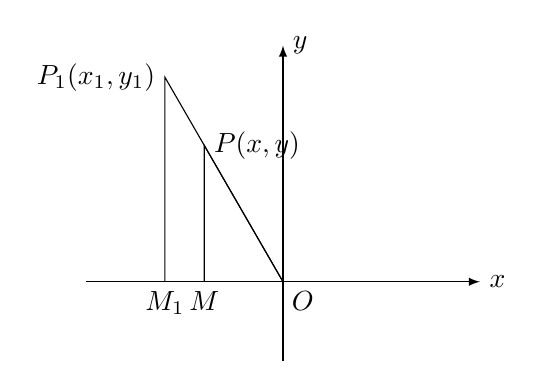
\begin{tikzpicture}[>=latex]
    \draw[->] (-2.5,0)--(2.5,0)node[right]{$x$};
    \draw[->] (0,-1)--(0,3)node[right]{$y$};
\draw (0,0)--(120:3)node[left]{$P_1(x_1,y_1)$}--(-1.5,0)node [below]{$M_1$};
\draw (0,0)--(120:2)node[right]{$P(x,y)$}--(-1,0)node [below]{$M$};
\node at (.25,-.25){$O$};
\end{tikzpicture}
